% =====================================================================
%  Relatório — 2ª Avaliação (Inteligência Artificial, CESAR School)
%  Formato IEEE de duas colunas (IEEEtran, conference)
%  Todos os números vêm de results/statistical_analysis.json e
%  results/metrics.csv da campanha campaign_full_30.
% =====================================================================
\documentclass[conference]{IEEEtran}

\usepackage[T1]{fontenc}
\usepackage[utf8]{inputenc}
\usepackage[brazil]{babel}
\usepackage{icomma}          % vírgula decimal em modo matemático
\usepackage{amsmath,amssymb}
\usepackage{graphicx}
\usepackage{booktabs}
\usepackage{cite}
\usepackage{url}
\usepackage[hidelinks]{hyperref}

\graphicspath{{figuras/}}
\renewcommand{\IEEEkeywordsname}{Palavras-chave}

\begin{document}

\title{Atenção Aditiva versus Atenção por Produto Escalar em Redes LSTM para Detecção de Spam em SMS: um Estudo Comparativo com 30 Simulações Pareadas}

% TODO: completar/ajustar a lista de autores do grupo
\author{
\IEEEauthorblockN{Eduardo Alves Lins}
\IEEEauthorblockA{CESAR School\\
Recife, PE, Brasil\\
eal3@cesar.school}
\and
\IEEEauthorblockN{Letícia da Silva}
\IEEEauthorblockA{CESAR School\\
Recife, PE, Brasil\\
\textit{[e-mail]}}
}

\maketitle

% ---------------------------------------------------------------------
\begin{abstract}
Este trabalho compara dois mecanismos de atenção --- o aditivo e o de produto escalar escalado --- acoplados a uma rede composta por \textit{embeddings} treináveis e uma LSTM, na tarefa de classificar mensagens SMS como \textit{spam} ou legítimas. Utilizou-se a base SMS Spam Collection (5.169 mensagens após a remoção de duplicatas) e um protocolo pareado de 30 simulações por cenário, no qual os dois modelos de cada par partem dos mesmos pesos iniciais nas camadas compartilhadas e recebem os lotes de treino na mesma ordem. A métrica principal foi o F1-score da classe \textit{spam}. A atenção aditiva obteve F1 de $0,9390 \pm 0,0103$ e a de produto escalar, $0,9373 \pm 0,0078$. As diferenças pareadas foram compatíveis com a normalidade (Shapiro--Wilk, $p = 0,81$) e o teste $t$ pareado não rejeitou a hipótese nula ($p = 0,48$; IC 95\,\% da diferença média $[-0,0033;\ 0,0068]$; $d_z = 0,13$), conclusão confirmada pelos testes de Wilcoxon e de permutação. Em análises exploratórias, a atenção aditiva apresentou recall e precisão média (\textit{average precision}) ligeiramente maiores, enquanto a de produto escalar treinou cerca de 11\,\% mais rápido. Conclui-se que, nesta configuração, não há evidência de diferença no F1 entre os mecanismos, e que o produto escalar entrega desempenho comparável com menor custo.
\end{abstract}

\begin{IEEEkeywords}
detecção de spam, LSTM, mecanismos de atenção, embeddings, teste de hipótese, aprendizado profundo
\end{IEEEkeywords}

% ---------------------------------------------------------------------
\section{Introdução}

Mensagens SMS indesejadas (\textit{spam}) incluem publicidade não solicitada, falsos prêmios e tentativas de golpe. Classificá-las automaticamente é um problema de classificação binária de textos curtos, ruidosos e com forte desbalanceamento entre classes~\cite{almeida2011}.

Redes neurais recorrentes do tipo LSTM~\cite{hochreiter1997} são uma escolha clássica para modelar sequências de palavras. Mecanismos de atenção~\cite{bahdanau2015,luong2015,vaswani2017} complementam a LSTM ao ponderar os estados ocultos de toda a sequência, construindo uma representação que enfatiza as posições mais relevantes para a decisão~\cite{yang2016}. Há, porém, diferentes formas de calcular esses pesos. A atenção \textbf{aditiva}~\cite{bahdanau2015} aprende projeções para comparar consulta e chaves; a atenção por \textbf{produto escalar escalado}~\cite{vaswani2017} compara os vetores diretamente, sem parâmetros adicionais.

Este trabalho investiga se essa escolha altera o desempenho de um classificador de \textit{spam}. Foram fixadas três técnicas --- (A)~\textit{embeddings} treináveis, (B)~LSTM e (C)~atenção --- e comparados dois cenários que diferem apenas na técnica~C:
\begin{itemize}
  \item \textbf{Cenário 1:} \textit{embeddings} + LSTM + atenção aditiva;
  \item \textbf{Cenário 2:} \textit{embeddings} + LSTM + atenção por produto escalar escalado.
\end{itemize}

As contribuições são: (i)~um protocolo experimental pareado com 30 simulações por cenário, que isola o efeito do mecanismo de atenção; (ii)~uma análise estatística com regra de decisão definida \textit{a priori}, acompanhada de tamanho de efeito e verificações de robustez; e (iii)~código e resultados abertos e reprodutíveis\footnote{\url{https://github.com/leticiagomesilva/spam-detection-study}}.

O restante do texto está organizado assim: a Seção~\ref{sec:fundamentacao} apresenta as técnicas; a Seção~\ref{sec:relacionados}, trabalhos relacionados; a Seção~\ref{sec:metodologia}, a metodologia; a Seção~\ref{sec:resultados}, os resultados; a Seção~\ref{sec:discussao} discute-os junto às limitações; e a Seção~\ref{sec:conclusao} conclui.

% ---------------------------------------------------------------------
\section{Fundamentação Teórica}
\label{sec:fundamentacao}

\subsection{Técnica A --- \textit{Embeddings}}
Cada token $x_t$ é mapeado para um vetor denso $\mathbf{e}_t = \mathbf{E}[x_t] \in \mathbb{R}^{d}$, em que $\mathbf{E}$ é uma matriz de \textit{embeddings} aprendida conjuntamente com o restante da rede. Diferentemente de representações esparsas, \textit{embeddings} posicionam palavras de uso semelhante em regiões próximas do espaço vetorial~\cite{mikolov2013}.

\subsection{Técnica B --- LSTM}
A LSTM~\cite{hochreiter1997} processa a sequência $\mathbf{e}_1,\dots,\mathbf{e}_T$ mantendo um estado de célula $\mathbf{c}_t$ controlado por portas de entrada ($\mathbf{i}_t$), esquecimento ($\mathbf{f}_t$) e saída ($\mathbf{o}_t$):
\begin{align}
\mathbf{i}_t &= \sigma(\mathbf{W}_i\mathbf{e}_t + \mathbf{U}_i\mathbf{h}_{t-1} + \mathbf{b}_i),\\
\mathbf{f}_t &= \sigma(\mathbf{W}_f\mathbf{e}_t + \mathbf{U}_f\mathbf{h}_{t-1} + \mathbf{b}_f),\\
\mathbf{o}_t &= \sigma(\mathbf{W}_o\mathbf{e}_t + \mathbf{U}_o\mathbf{h}_{t-1} + \mathbf{b}_o),\\
\tilde{\mathbf{c}}_t &= \tanh(\mathbf{W}_c\mathbf{e}_t + \mathbf{U}_c\mathbf{h}_{t-1} + \mathbf{b}_c),\\
\mathbf{c}_t &= \mathbf{f}_t \odot \mathbf{c}_{t-1} + \mathbf{i}_t \odot \tilde{\mathbf{c}}_t,\\
\mathbf{h}_t &= \mathbf{o}_t \odot \tanh(\mathbf{c}_t).
\end{align}
As portas permitem preservar informação por muitos passos, mitigando o desaparecimento do gradiente.

\subsection{Técnica C --- Mecanismos de Atenção}
Seja $\mathbf{H} = [\mathbf{h}_1,\dots,\mathbf{h}_T]$ a sequência de estados ocultos e $\mathbf{q} = \mathbf{h}_T$ o último estado válido (consulta). A atenção atribui um escore $s_i$ a cada posição, normaliza-os e produz um vetor de contexto:
\begin{equation}
\alpha_i = \frac{\exp(s_i)}{\sum_{j=1}^{T}\exp(s_j)}, \qquad \mathbf{c} = \sum_{i=1}^{T}\alpha_i\,\mathbf{h}_i .
\end{equation}
Os dois cenários diferem apenas na função de escore.

\textbf{Atenção aditiva}~\cite{bahdanau2015}:
\begin{equation}
s_i = \mathbf{v}^{\top}\tanh(\mathbf{W}_q\mathbf{q} + \mathbf{W}_k\mathbf{h}_i),
\end{equation}
com $\mathbf{W}_q,\mathbf{W}_k \in \mathbb{R}^{d_a \times d_h}$ e $\mathbf{v} \in \mathbb{R}^{d_a}$ treináveis. Com $d_h = d_a = 64$, são $2 \cdot 64 \cdot 64 + 64 = 8.256$ parâmetros adicionais.

\textbf{Atenção por produto escalar escalado}~\cite{luong2015,vaswani2017}:
\begin{equation}
s_i = \frac{\mathbf{q}^{\top}\mathbf{h}_i}{\sqrt{d_h}},
\end{equation}
sem parâmetros adicionais. O fator $\sqrt{d_h}$ evita escores muito grandes, que saturariam o \textit{softmax}.

% ---------------------------------------------------------------------
\section{Trabalhos Relacionados}
\label{sec:relacionados}

Almeida \textit{et al.}~\cite{almeida2011} disponibilizaram a SMS Spam Collection~\cite{uci_sms} e avaliaram classificadores tradicionais sobre ela, estabelecendo a base como referência para o problema. Em classificação de documentos, Yang \textit{et al.}~\cite{yang2016} mostraram que a atenção sobre estados de redes recorrentes melhora o desempenho e oferece pesos interpretáveis, ainda que Jain e Wallace~\cite{jain2019} alertem que esses pesos não constituem, por si só, explicações fiéis do modelo. Luong \textit{et al.}~\cite{luong2015} compararam diferentes funções de escore (incluindo a aditiva e o produto escalar) em tradução automática, e Vaswani \textit{et al.}~\cite{vaswani2017} popularizaram a versão escalada do produto escalar.

Quanto à metodologia de comparação, Dietterich~\cite{dietterich1998} e Demšar~\cite{demsar2006} discutem testes estatísticos para comparar classificadores, recomendando atenção às premissas dos testes e o uso de alternativas não paramétricas quando necessário --- orientação seguida neste estudo.

% ---------------------------------------------------------------------
\section{Metodologia}
\label{sec:metodologia}

\subsection{Base de Dados}
Utilizou-se a SMS Spam Collection v.1~\cite{uci_sms}, com 5.572 mensagens em inglês rotuladas como \textit{ham} (legítima) ou \textit{spam}. Antes de qualquer divisão, removeram-se 403 duplicatas exatas (mesmo texto e mesmo rótulo), mantendo a primeira ocorrência; não houve textos repetidos com rótulos conflitantes. A base resultante foi dividida de forma estratificada em treino, validação e teste (70/15/15\,\%, semente 42), uma única vez para todo o estudo (Tabela~\ref{tab:dados}). A remoção prévia das duplicatas impede que a mesma mensagem apareça em partições diferentes.

\begin{table}[!t]
\caption{Composição da base de dados}
\label{tab:dados}
\centering
\footnotesize
\begin{tabular}{lrrr}
\toprule
Conjunto & \textit{Ham} & \textit{Spam} & Total \\
\midrule
Original                & 4.825 & 747 & 5.572 \\
Após deduplicação       & 4.516 & 653 & 5.169 \\
\midrule
Treino (70\,\%)         & --- & --- & 3.618 \\
Validação (15\,\%)      & --- & --- & 775 \\
Teste (15\,\%)          & 678 & 98 & 776 \\
\bottomrule
\end{tabular}
\end{table}

\subsection{Pré-processamento}
Os textos foram convertidos para minúsculas e tokenizados com o \texttt{Tokenizer} do Keras, ajustado \textbf{somente} sobre o conjunto de treino (7.335 tokens distintos; limite de 10.000), com token especial para palavras fora do vocabulário. Validação e teste foram apenas transformados. Com o filtro padrão do \texttt{Tokenizer}, a maior parte da pontuação (como ``!'', ``\$'', ``@'', ponto e barra) é removida na tokenização; dígitos, apóstrofos e o símbolo ``\pounds'' são mantidos, e URLs são fragmentadas em partes (por exemplo, \texttt{http}, \texttt{www}, \texttt{com}). As sequências foram truncadas ou completadas com zeros à direita até 100 tokens. O índice zero é reservado ao preenchimento e gera uma máscara propagada à LSTM e à camada de atenção.

\subsection{Arquitetura}
Ambos os cenários usam a mesma arquitetura, exceto pela camada de atenção: \textit{Embedding} (64 dimensões, com máscara) $\rightarrow$ LSTM (64 unidades, retornando todos os estados) $\rightarrow$ atenção (aditiva ou produto escalar), tendo como consulta o último estado válido $\mathbf{h}_T$ $\rightarrow$ \textit{Dropout}~\cite{srivastava2014} (0,2) $\rightarrow$ camada densa com ativação sigmoide. Nas posições de preenchimento, soma-se $-10^{9}$ ao escore antes do \textit{softmax}, anulando seus pesos. O modelo com atenção por produto escalar tem 673.153 parâmetros treináveis e o com atenção aditiva, 681.409 (+1,2\,\%). A Tabela~\ref{tab:hiper} resume os hiperparâmetros, idênticos nos dois cenários.

\begin{table}[!t]
\caption{Hiperparâmetros (comuns aos dois cenários)}
\label{tab:hiper}
\centering
\footnotesize
\begin{tabular}{ll}
\toprule
Parâmetro & Valor \\
\midrule
Dimensão do \textit{embedding} & 64 \\
Unidades da LSTM & 64 \\
Dimensão interna da atenção aditiva & 64 \\
\textit{Dropout} & 0,2 \\
Comprimento máximo da sequência & 100 tokens \\
Otimizador & Adam~\cite{kingma2015}, taxa 0,001 \\
Função de perda & entropia cruzada binária \\
Tamanho do lote & 32 \\
Épocas (máximo) & 20 \\
Parada antecipada & \texttt{val\_loss}, paciência 3, melhores pesos \\
Limiar de decisão & 0,5 \\
\bottomrule
\end{tabular}
\end{table}

\subsection{Protocolo Experimental Pareado}
Foram realizadas 30 simulações por cenário (60 treinamentos), indexadas pelas sementes $k \in \{1001,\dots,1030\}$. Para cada $k$:
\begin{enumerate}
  \item o modelo com atenção aditiva é inicializado com a semente $k$;
  \item o modelo com produto escalar é construído e recebe uma \textbf{cópia exata} dos pesos das camadas compartilhadas (\textit{embedding}, LSTM e saída), verificada numericamente;
  \item os dados de treino são embaralhados \textbf{uma única vez} com a semente $k$, e ambos os modelos são treinados com a mesma sequência de lotes em todas as épocas;
  \item ambos são avaliados no mesmo conjunto de teste, usado apenas na avaliação final.
\end{enumerate}
Assim, os dois modelos de um par diferem somente no mecanismo de atenção, e a variabilidade entre pares reflete a inicialização e a ordem dos lotes. O determinismo de operações do TensorFlow~\cite{tensorflow} foi ativado. Os experimentos foram executados em CPU (Intel, 16 núcleos; Windows~11; Python~3.11.9; TensorFlow~2.15.0), e a campanha completa levou 28~min~44~s.

\subsection{Métricas}
A métrica principal é o \textbf{F1-score da classe \textit{spam}}, adequado ao desbalanceamento (12,6\,\% de \textit{spam}). Como métricas complementares, foram registradas a precisão e o recall da classe \textit{spam}, a acurácia, a precisão média (\textit{average precision}, AP, independente de limiar), a matriz de confusão e o tempo de treino.

\subsection{Análise Estatística}
Para cada par $k$, define-se $d_k = \mathrm{F1}_{\text{aditiva},k} - \mathrm{F1}_{\text{produto},k}$. As hipóteses são:
\begin{itemize}
  \item $H_0$: $\mathbb{E}[d] = 0$ (não há diferença no F1 esperado);
  \item $H_1$: $\mathbb{E}[d] \neq 0$ (há diferença no F1 esperado).
\end{itemize}
A regra de decisão foi definida antes da análise, com $\alpha = 0,05$: aplica-se o teste de Shapiro--Wilk~\cite{shapiro1965} às 30 diferenças; se a normalidade não for rejeitada, usa-se o teste $t$ pareado bilateral; caso contrário, o teste de postos sinalizados de Wilcoxon~\cite{wilcoxon1945}. Como verificações de robustez, independentes de distribuição, reportam-se um teste de permutação pareado por troca de sinais (10.000 permutações)~\cite{good2005} e um intervalo de confiança \textit{bootstrap} percentil de 95\,\% (10.000 reamostras)~\cite{efron1993}. O tamanho de efeito é medido pelo $d_z$ de Cohen ($\bar{d}/s_d$)~\cite{cohen1988} e pela correlação rank-biserial pareada $r_{rb}$~\cite{kerby2014}. As métricas secundárias passaram pelo mesmo procedimento, em caráter exploratório e sem correção para comparações múltiplas.

% ---------------------------------------------------------------------
\section{Resultados}
\label{sec:resultados}

\subsection{Desempenho de Classificação}
A Tabela~\ref{tab:metricas} resume as métricas no conjunto de teste ao longo das 30 simulações. Os dois cenários atingem desempenho elevado e muito próximo: a diferença média de F1 é de $0,0017$, menor do que o desvio padrão de qualquer um dos cenários. As Figs.~\ref{fig:f1dist} e~\ref{fig:metricas} mostram a sobreposição das distribuições.

\begin{table}[!t]
\caption{Métricas no conjunto de teste (média $\pm$ desvio padrão, 30 simulações)}
\label{tab:metricas}
\centering
\footnotesize
\setlength{\tabcolsep}{4pt}
\begin{tabular}{lcc}
\toprule
Métrica & Aditiva & Produto escalar \\
\midrule
\textbf{F1 (\textit{spam})} & $\mathbf{0,9390 \pm 0,0103}$ & $\mathbf{0,9373 \pm 0,0078}$ \\
Precisão (\textit{spam})     & $0,9289 \pm 0,0216$ & $0,9320 \pm 0,0144$ \\
Recall (\textit{spam})       & $0,9500 \pm 0,0157$ & $0,9429 \pm 0,0106$ \\
Acurácia                     & $0,9844 \pm 0,0028$ & $0,9841 \pm 0,0020$ \\
\textit{Average precision}   & $0,9816 \pm 0,0027$ & $0,9777 \pm 0,0023$ \\
Tempo de treino (s)          & $28,90 \pm 5,74$    & $25,70 \pm 5,15$ \\
Épocas executadas            & $6,83 \pm 1,56$     & $6,30 \pm 1,51$ \\
\bottomrule
\end{tabular}
\end{table}

\begin{figure}[!t]
\centering
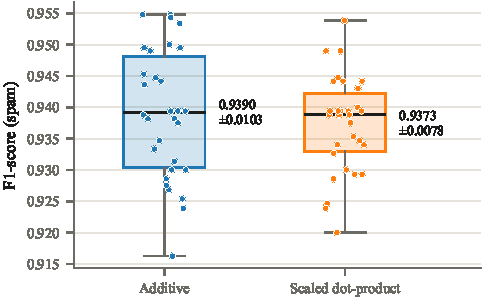
\includegraphics[width=\columnwidth]{fig_f1_distribution.pdf}
\caption{Distribuição do F1-score da classe \textit{spam} nas 30 simulações de cada cenário. Cada ponto é uma semente; o texto indica média $\pm$ desvio padrão.}
\label{fig:f1dist}
\end{figure}

\begin{figure}[!t]
\centering
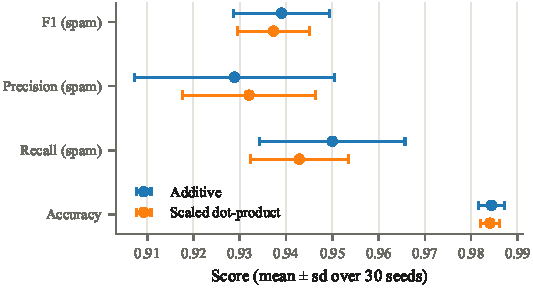
\includegraphics[width=\columnwidth]{fig_metrics.pdf}
\caption{Média $\pm$ desvio padrão das métricas de classificação por cenário. O eixo não começa em zero para tornar visíveis as diferenças.}
\label{fig:metricas}
\end{figure}

\subsection{Teste de Hipótese (F1)}
A Tabela~\ref{tab:teste} apresenta a análise da métrica principal. O teste de Shapiro--Wilk não rejeitou a normalidade das diferenças ($W = 0,979$; $p = 0,810$), o que é corroborado pelo gráfico Q-Q (Fig.~\ref{fig:qq}); pela regra pré-definida, aplicou-se o teste $t$ pareado. O resultado, $t(29) = 0,713$ e $p = 0,481$, \textbf{não permite rejeitar $H_0$}. O intervalo de confiança de 95\,\% da diferença média, $[-0,0033;\ 0,0068]$, contém o zero, e o tamanho de efeito é desprezível ($d_z = 0,13$). Os testes de Wilcoxon ($p = 0,543$) e de permutação ($p = 0,475$), bem como o intervalo \textit{bootstrap}, levam à mesma conclusão.

A Fig.~\ref{fig:dif} mostra o histograma das diferenças, centrado próximo de zero e com valores positivos e negativos. Na Fig.~\ref{fig:pareado}, as linhas que ligam os resultados de uma mesma semente se cruzam em ambas as direções: a atenção aditiva superou a de produto escalar em 16 pares e foi inferior em 14.

\begin{table}[!t]
\caption{Análise estatística do F1 ($d = \mathrm{F1}_{\text{aditiva}} - \mathrm{F1}_{\text{produto}}$, $n = 30$)}
\label{tab:teste}
\centering
\footnotesize
\begin{tabular}{ll}
\toprule
Procedimento & Resultado \\
\midrule
Diferença média ($\pm$ desvio)   & $0,0017 \pm 0,0134$ \\
Shapiro--Wilk                    & $W = 0,979$; $p = 0,810$ (normal) \\
\textbf{Teste $t$ pareado}       & $\mathbf{t(29) = 0,713}$; $\mathbf{p = 0,481}$ \\
IC 95\,\% ($t$)                  & $[-0,0033;\ 0,0068]$ \\
Wilcoxon                         & $W = 201,5$; $p = 0,543$ \\
Permutação (10.000)              & $p = 0,475$ \\
IC 95\,\% \textit{bootstrap}     & $[-0,0028;\ 0,0064]$ \\
$d_z$ de Cohen                   & $0,130$ (desprezível) \\
Rank-biserial $r_{rb}$           & $0,133$ \\
\midrule
\textbf{Decisão} ($\alpha = 0,05$) & \textbf{não rejeitar $H_0$} \\
\bottomrule
\end{tabular}
\end{table}

\begin{figure}[!t]
\centering
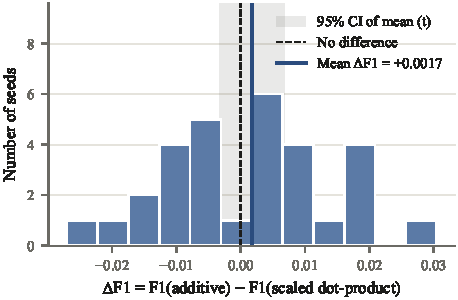
\includegraphics[width=\columnwidth]{fig_f1_differences.pdf}
\caption{Histograma das diferenças pareadas de F1. A faixa cinza é o IC de 95\,\% da diferença média (teste $t$), que contém o zero.}
\label{fig:dif}
\end{figure}

\begin{figure}[!t]
\centering
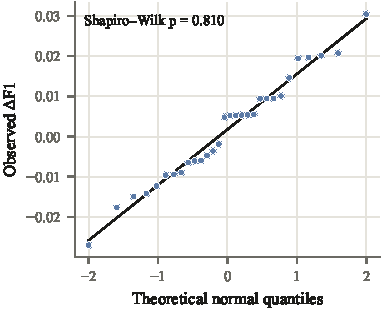
\includegraphics[width=0.75\columnwidth]{fig_qq.pdf}
\caption{Gráfico Q-Q normal das diferenças de F1, que apoia a escolha do teste $t$ pareado.}
\label{fig:qq}
\end{figure}

\begin{figure}[!t]
\centering
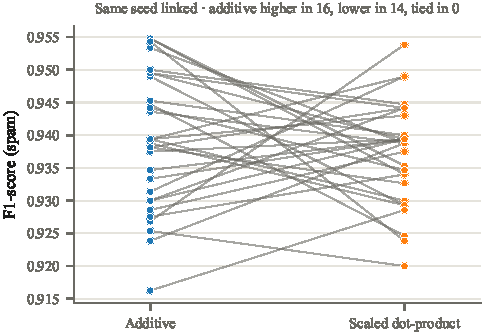
\includegraphics[width=\columnwidth]{fig_f1_paired.pdf}
\caption{F1 de cada semente nos dois cenários; as linhas ligam os modelos de um mesmo par.}
\label{fig:pareado}
\end{figure}

\subsection{Métricas Secundárias}
A Tabela~\ref{tab:secundarias} aplica o mesmo procedimento às demais métricas. Não houve diferença em precisão nem em acurácia. Para a precisão, a normalidade foi rejeitada ($p = 0,033$), o que levou ao teste de Wilcoxon; a estatística $W = 231,5$ ficou praticamente no seu valor esperado sob $H_0$ ($232,5$), resultando em $p \approx 1$. A atenção aditiva obteve recall maior ($+0,0071$; $p = 0,017$; $d_z = 0,46$) e \textit{average precision} maior ($+0,0039$; $p < 0,001$; $d_z = 1,31$). Em termos absolutos, porém, essas diferenças são pequenas: com 98 mensagens de \textit{spam} no teste, $+0,0071$ de recall equivale a cerca de 0,7 mensagem a mais detectada por simulação. A matriz de confusão média (Fig.~\ref{fig:confusao}) confirma esse quadro: 4,9 contra 5,6 falsos negativos e 7,2 contra 6,8 falsos positivos.

\begin{table}[!t]
\caption{Métricas secundárias (exploratórias; $\Delta$ = aditiva $-$ produto escalar)}
\label{tab:secundarias}
\centering
\footnotesize
\setlength{\tabcolsep}{3.5pt}
\begin{tabular}{lrlrl}
\toprule
Métrica & $\Delta$ médio & Teste & $p$ & Resultado \\
\midrule
Precisão            & $-0,0032$ & Wilcoxon & $1,000$  & n.s. \\
Recall              & $+0,0071$ & $t$      & $0,017$  & aditiva \\
Acurácia            & $+0,0003$ & $t$      & $0,606$  & n.s. \\
\textit{Avg. precision} & $+0,0039$ & $t$  & $<0,001$ & aditiva \\
Tempo (s)           & $+3,20$   & $t$      & $0,025$  & produto \\
\bottomrule
\multicolumn{5}{l}{\scriptsize n.s.: não significativo a $\alpha = 0,05$. ``Resultado'' indica o cenário favorecido.}
\end{tabular}
\end{table}

\begin{figure}[!t]
\centering
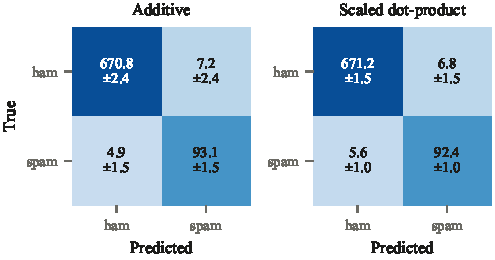
\includegraphics[width=\columnwidth]{fig_confusion.pdf}
\caption{Matriz de confusão média ($\pm$ desvio padrão) no conjunto de teste (678 \textit{ham}, 98 \textit{spam}). A cor usa escala logarítmica para tornar visíveis as células pequenas.}
\label{fig:confusao}
\end{figure}

\subsection{Custo Computacional e Convergência}
A atenção por produto escalar treinou em média $25,70$~s contra $28,90$~s da aditiva ($-11\,\%$; $p = 0,025$; $d_z = 0,43$). A diferença decorre de dois fatores (Fig.~\ref{fig:tempo}): um custo por época ligeiramente menor ($4,11$ contra $4,26$~s, ou $-3,3\,\%$), coerente com a ausência das projeções $\mathbf{W}_q$, $\mathbf{W}_k$ e $\mathbf{v}$; e uma parada antecipada um pouco mais cedo ($6,30$ contra $6,83$ épocas). As curvas de perda (Fig.~\ref{fig:curvas}) são praticamente sobrepostas: ambos os modelos atingem a menor perda de validação por volta da terceira ou quarta época, após a qual a perda de treino continua a cair sem ganho na validação.

\begin{figure}[!t]
\centering
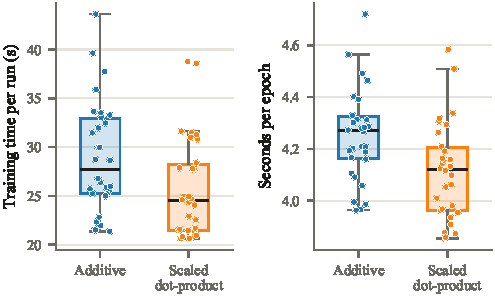
\includegraphics[width=\columnwidth]{fig_train_time.pdf}
\caption{Tempo total de treino por simulação (esq.) e tempo por época (dir.).}
\label{fig:tempo}
\end{figure}

\begin{figure}[!t]
\centering
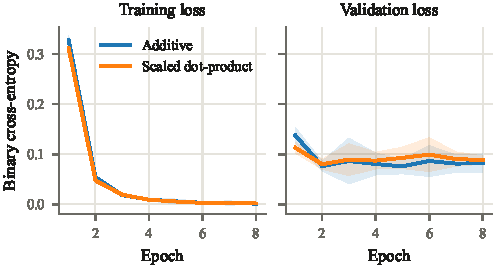
\includegraphics[width=\columnwidth]{fig_learning_curves.pdf}
\caption{Perda média ($\pm$ desvio padrão) por época nas 30 simulações. As curvas são exibidas enquanto ao menos cinco simulações ainda estavam em treinamento.}
\label{fig:curvas}
\end{figure}

\subsection{Análise Qualitativa da Atenção}
A Fig.~\ref{fig:atencao} mostra os pesos de atenção de ambos os modelos da semente 1001 em três mensagens de teste corretamente classificadas. Nesses exemplos, a atenção aditiva concentra o maior peso nos tokens finais da mensagem (máximos entre 0,13 e 0,21, sempre no último token), enquanto a de produto escalar distribui os pesos de forma mais uniforme (máximos de cerca de 0,11). Uma explicação plausível é que a consulta é o último estado $\mathbf{h}_T$, naturalmente mais semelhante aos estados vizinhos; a atenção aditiva, que aprende como comparar, parece reforçar essa tendência. Trata-se de uma ilustração: pesos de atenção não devem ser lidos como explicação causal da decisão~\cite{jain2019}.

\begin{figure*}[!t]
\centering
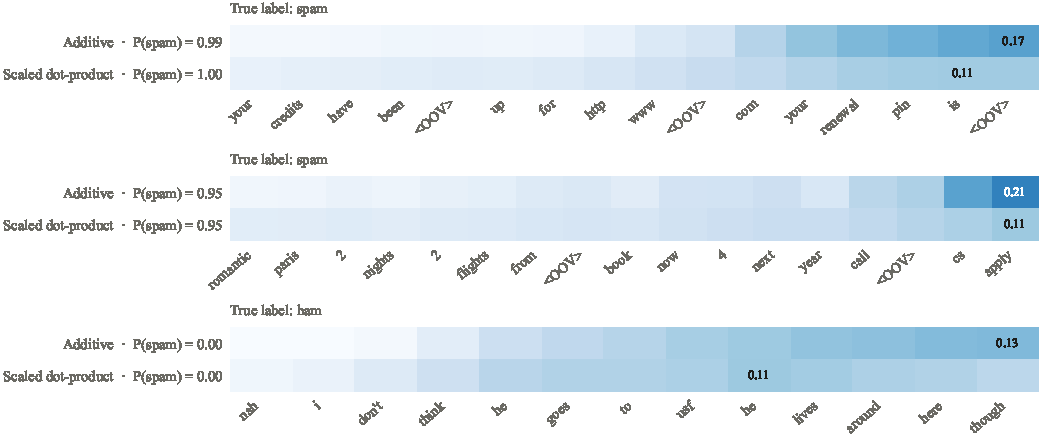
\includegraphics[width=\textwidth]{fig_attention.pdf}
\caption{Pesos de atenção dos dois mecanismos (semente 1001) em três mensagens do conjunto de teste. Cores mais escuras indicam maior peso; o número marca o maior peso de cada linha. P(\textit{spam}) é a probabilidade prevista pelo modelo. \texttt{<OOV>} indica um token fora do vocabulário.}
\label{fig:atencao}
\end{figure*}

% ---------------------------------------------------------------------
\section{Discussão}
\label{sec:discussao}

\subsection{Qual abordagem é mais eficaz?}
Na métrica principal, os dados \textbf{não permitem rejeitar a hipótese nula}: não há evidência de diferença no F1 esperado entre os dois mecanismos de atenção. A diferença média observada ($0,0017$) é inferior ao efeito de uma única mensagem classificada de forma diferente --- com 98 mensagens de \textit{spam} no teste, uma mensagem altera o F1 em cerca de $0,005$ a $0,01$. Ambos os modelos operam próximos do limite de desempenho desta base, o que deixa pouco espaço para que a técnica~C faça diferença.

As análises exploratórias sugerem que a atenção aditiva ordena um pouco melhor as mensagens por probabilidade de \textit{spam} (AP maior em 27 dos 30 pares, $d_z = 1,31$) e recupera ligeiramente mais \textit{spam} (recall), ao custo de 8.256 parâmetros adicionais e de cerca de 11\,\% mais tempo de treino. Essas diferenças são pequenas em termos absolutos e, por não terem sido corrigidas para comparações múltiplas, devem ser tratadas como hipóteses para estudos futuros. Do ponto de vista prático, a atenção por produto escalar entrega F1 equivalente com menor custo e menos parâmetros; a aditiva só se justificaria se o recall fosse prioridade explícita.

\subsection{Limitações}
\begin{enumerate}
  \item \textbf{Divisão única:} as 30 simulações compartilham a mesma partição treino/validação/teste. Elas medem a variabilidade do treinamento (inicialização e ordem dos lotes), e não a variação entre amostras de mensagens; generalizações além desta partição exigiriam validação cruzada.
  \item \textbf{Não rejeitar $H_0$ não prova equivalência.} Para afirmar equivalência seria necessário um teste de equivalência (por exemplo, TOST~\cite{lakens2017}) com uma margem definida previamente.
  \item \textbf{Pré-processamento:} o filtro padrão do tokenizador removeu a maior parte da pontuação e fragmentou URLs, descartando sinais potencialmente úteis. O efeito é idêntico nos dois cenários e não compromete a comparação, mas pode limitar o desempenho absoluto.
  \item \textbf{Base de dados:} uma única base, pequena, em inglês e de 2011; os padrões de \textit{spam} atuais podem ser diferentes.
  \item \textbf{Tempo de treino:} medido em CPU, com o modelo aditivo sempre treinado primeiro dentro de cada par; efeitos de ordem não podem ser descartados.
  \item \textbf{Hiperparâmetros:} fixados e iguais para os dois cenários, sem ajuste específico para cada mecanismo.
\end{enumerate}

% ---------------------------------------------------------------------
\section{Conclusão}
\label{sec:conclusao}

Este trabalho comparou as atenções aditiva e por produto escalar escalado em um classificador de \textit{spam} baseado em \textit{embeddings} e LSTM, por meio de 30 simulações pareadas por cenário. Com F1 de $0,9390 \pm 0,0103$ (aditiva) e $0,9373 \pm 0,0078$ (produto escalar) e um teste $t$ pareado com $p = 0,481$, \textbf{a hipótese nula não foi rejeitada}: não há evidência de que um mecanismo seja mais eficaz do que o outro em F1. A atenção aditiva mostrou pequenas vantagens exploratórias em recall e \textit{average precision}, enquanto a de produto escalar foi cerca de 11\,\% mais rápida e não acrescenta parâmetros. Nesta configuração, portanto, o produto escalar oferece o melhor equilíbrio entre desempenho e custo.

Como trabalhos futuros, propõem-se: validação cruzada com múltiplas partições; um teste de equivalência com margem definida previamente; a preservação da pontuação e das URLs na tokenização; o uso de \textit{embeddings} pré-treinados e de LSTMs bidirecionais; e a avaliação em bases mais recentes e em português.

% ---------------------------------------------------------------------
\begin{thebibliography}{99}

\bibitem{almeida2011}
T.~A. Almeida, J.~M.~G. Hidalgo, and A.~Yamakami, ``Contributions to the study of SMS spam filtering: New collection and results,'' in \textit{Proc. 11th ACM Symp. Document Engineering (DocEng)}, Mountain View, CA, USA, 2011, pp.~259--262.

\bibitem{uci_sms}
T.~A. Almeida and J.~M.~G. Hidalgo, ``SMS Spam Collection,'' UCI Machine Learning Repository, 2011. [Online]. Available: \url{https://archive.ics.uci.edu/dataset/228/sms+spam+collection}

\bibitem{hochreiter1997}
S.~Hochreiter and J.~Schmidhuber, ``Long short-term memory,'' \textit{Neural Computation}, vol.~9, no.~8, pp.~1735--1780, 1997.

\bibitem{mikolov2013}
T.~Mikolov, I.~Sutskever, K.~Chen, G.~S. Corrado, and J.~Dean, ``Distributed representations of words and phrases and their compositionality,'' in \textit{Advances in Neural Information Processing Systems (NIPS)}, 2013, pp.~3111--3119.

\bibitem{bahdanau2015}
D.~Bahdanau, K.~Cho, and Y.~Bengio, ``Neural machine translation by jointly learning to align and translate,'' in \textit{Proc. Int. Conf. Learning Representations (ICLR)}, 2015.

\bibitem{luong2015}
M.-T. Luong, H.~Pham, and C.~D. Manning, ``Effective approaches to attention-based neural machine translation,'' in \textit{Proc. Conf. Empirical Methods in Natural Language Processing (EMNLP)}, 2015, pp.~1412--1421.

\bibitem{vaswani2017}
A.~Vaswani \textit{et al.}, ``Attention is all you need,'' in \textit{Advances in Neural Information Processing Systems (NIPS)}, 2017, pp.~5998--6008.

\bibitem{yang2016}
Z.~Yang, D.~Yang, C.~Dyer, X.~He, A.~Smola, and E.~Hovy, ``Hierarchical attention networks for document classification,'' in \textit{Proc. NAACL-HLT}, 2016, pp.~1480--1489.

\bibitem{jain2019}
S.~Jain and B.~C. Wallace, ``Attention is not explanation,'' in \textit{Proc. NAACL-HLT}, 2019, pp.~3543--3556.

\bibitem{dietterich1998}
T.~G. Dietterich, ``Approximate statistical tests for comparing supervised classification learning algorithms,'' \textit{Neural Computation}, vol.~10, no.~7, pp.~1895--1923, 1998.

\bibitem{demsar2006}
J.~Demšar, ``Statistical comparisons of classifiers over multiple data sets,'' \textit{J. Machine Learning Research}, vol.~7, pp.~1--30, 2006.

\bibitem{srivastava2014}
N.~Srivastava, G.~Hinton, A.~Krizhevsky, I.~Sutskever, and R.~Salakhutdinov, ``Dropout: A simple way to prevent neural networks from overfitting,'' \textit{J. Machine Learning Research}, vol.~15, pp.~1929--1958, 2014.

\bibitem{kingma2015}
D.~P. Kingma and J.~Ba, ``Adam: A method for stochastic optimization,'' in \textit{Proc. Int. Conf. Learning Representations (ICLR)}, 2015.

\bibitem{tensorflow}
M.~Abadi \textit{et al.}, ``TensorFlow: Large-scale machine learning on heterogeneous systems,'' 2015. [Online]. Available: \url{https://www.tensorflow.org}

\bibitem{shapiro1965}
S.~S. Shapiro and M.~B. Wilk, ``An analysis of variance test for normality (complete samples),'' \textit{Biometrika}, vol.~52, no.~3/4, pp.~591--611, 1965.

\bibitem{wilcoxon1945}
F.~Wilcoxon, ``Individual comparisons by ranking methods,'' \textit{Biometrics Bulletin}, vol.~1, no.~6, pp.~80--83, 1945.

\bibitem{good2005}
P.~Good, \textit{Permutation, Parametric, and Bootstrap Tests of Hypotheses}, 3rd~ed. New York, NY, USA: Springer, 2005.

\bibitem{efron1993}
B.~Efron and R.~J. Tibshirani, \textit{An Introduction to the Bootstrap}. New York, NY, USA: Chapman \& Hall, 1993.

\bibitem{cohen1988}
J.~Cohen, \textit{Statistical Power Analysis for the Behavioral Sciences}, 2nd~ed. Hillsdale, NJ, USA: Lawrence Erlbaum, 1988.

\bibitem{kerby2014}
D.~S. Kerby, ``The simple difference formula: An approach to teaching nonparametric correlation,'' \textit{Comprehensive Psychology}, vol.~3, 2014.

\bibitem{lakens2017}
D.~Lakens, ``Equivalence tests: A practical primer for $t$ tests, correlations, and meta-analyses,'' \textit{Social Psychological and Personality Science}, vol.~8, no.~4, pp.~355--362, 2017.

\end{thebibliography}

\end{document}
